\chapter{Method}

\section{Data Collection}
\label{sec:data}
The experiment was hosted through an open-source crowdsourcing client/system server system LingoTurk \cite{lingoturk}.
While the participants were recruited via Prolific \cite{prolific} - a subject pool for online experiments. The following criteria were used to filter the participants: native English speaker located in the UK, age in range 18-40, minimal approval rate of 95\%, number of previous submissions must be ar least 20 studies, participants cannot have taken part in any of the related studies our group has conducted before. The estimated length of the experiment was 22 minutes, while the actual median was 19 minutes 30 seconds. The participants were paid 3.89 pounds which is equivalent to minimal hour wage in Germany. The participants were paid only in case of successful completion of the full experiment. The experiment was conducted in a web browser and the participants were asked to use a computer with functional webcam. 


\subsection{Reference Games}
\label{sec:data:ref_games}
There are 3 conditions of the reference games: Simple, Complex and Unambiguous. In the \autoref{sec:rsa} we mainly talked about the Simple and Complex conditions. The Unambiguous condition suits two main purposes. First of all, it acts as a sort of filler, so that participants do not get used to the same type of problems. Second of all, it acts as a control check, that is, participants who do not reach over 50\% accuracy on the Unambiguous trials are excluded from the analysis.

The trials were generated using 3 colors: red, green and blue, and 3 shapes: square, circle and triangle. In total there are 72 combinations of unique trials. The full list of trials can be found \TODO{insert link to apendix}. The code used to generate trials can be found at \TODO{insert link to the source code} For each condition every unique sent message was repeated exactly twice. Which results in 12 trials of every condition. Furthermore one simple and one complex trial was picked to be repeated once again in the very end of the experiment. These were so called strategy trials where we would ask the participants to explain their reasoning behind the choice of the object. All trials were randomly shuffled before the experiment, except for the strategy trials which were always at the end of the experiment.

\begin{figure}
    \centering
    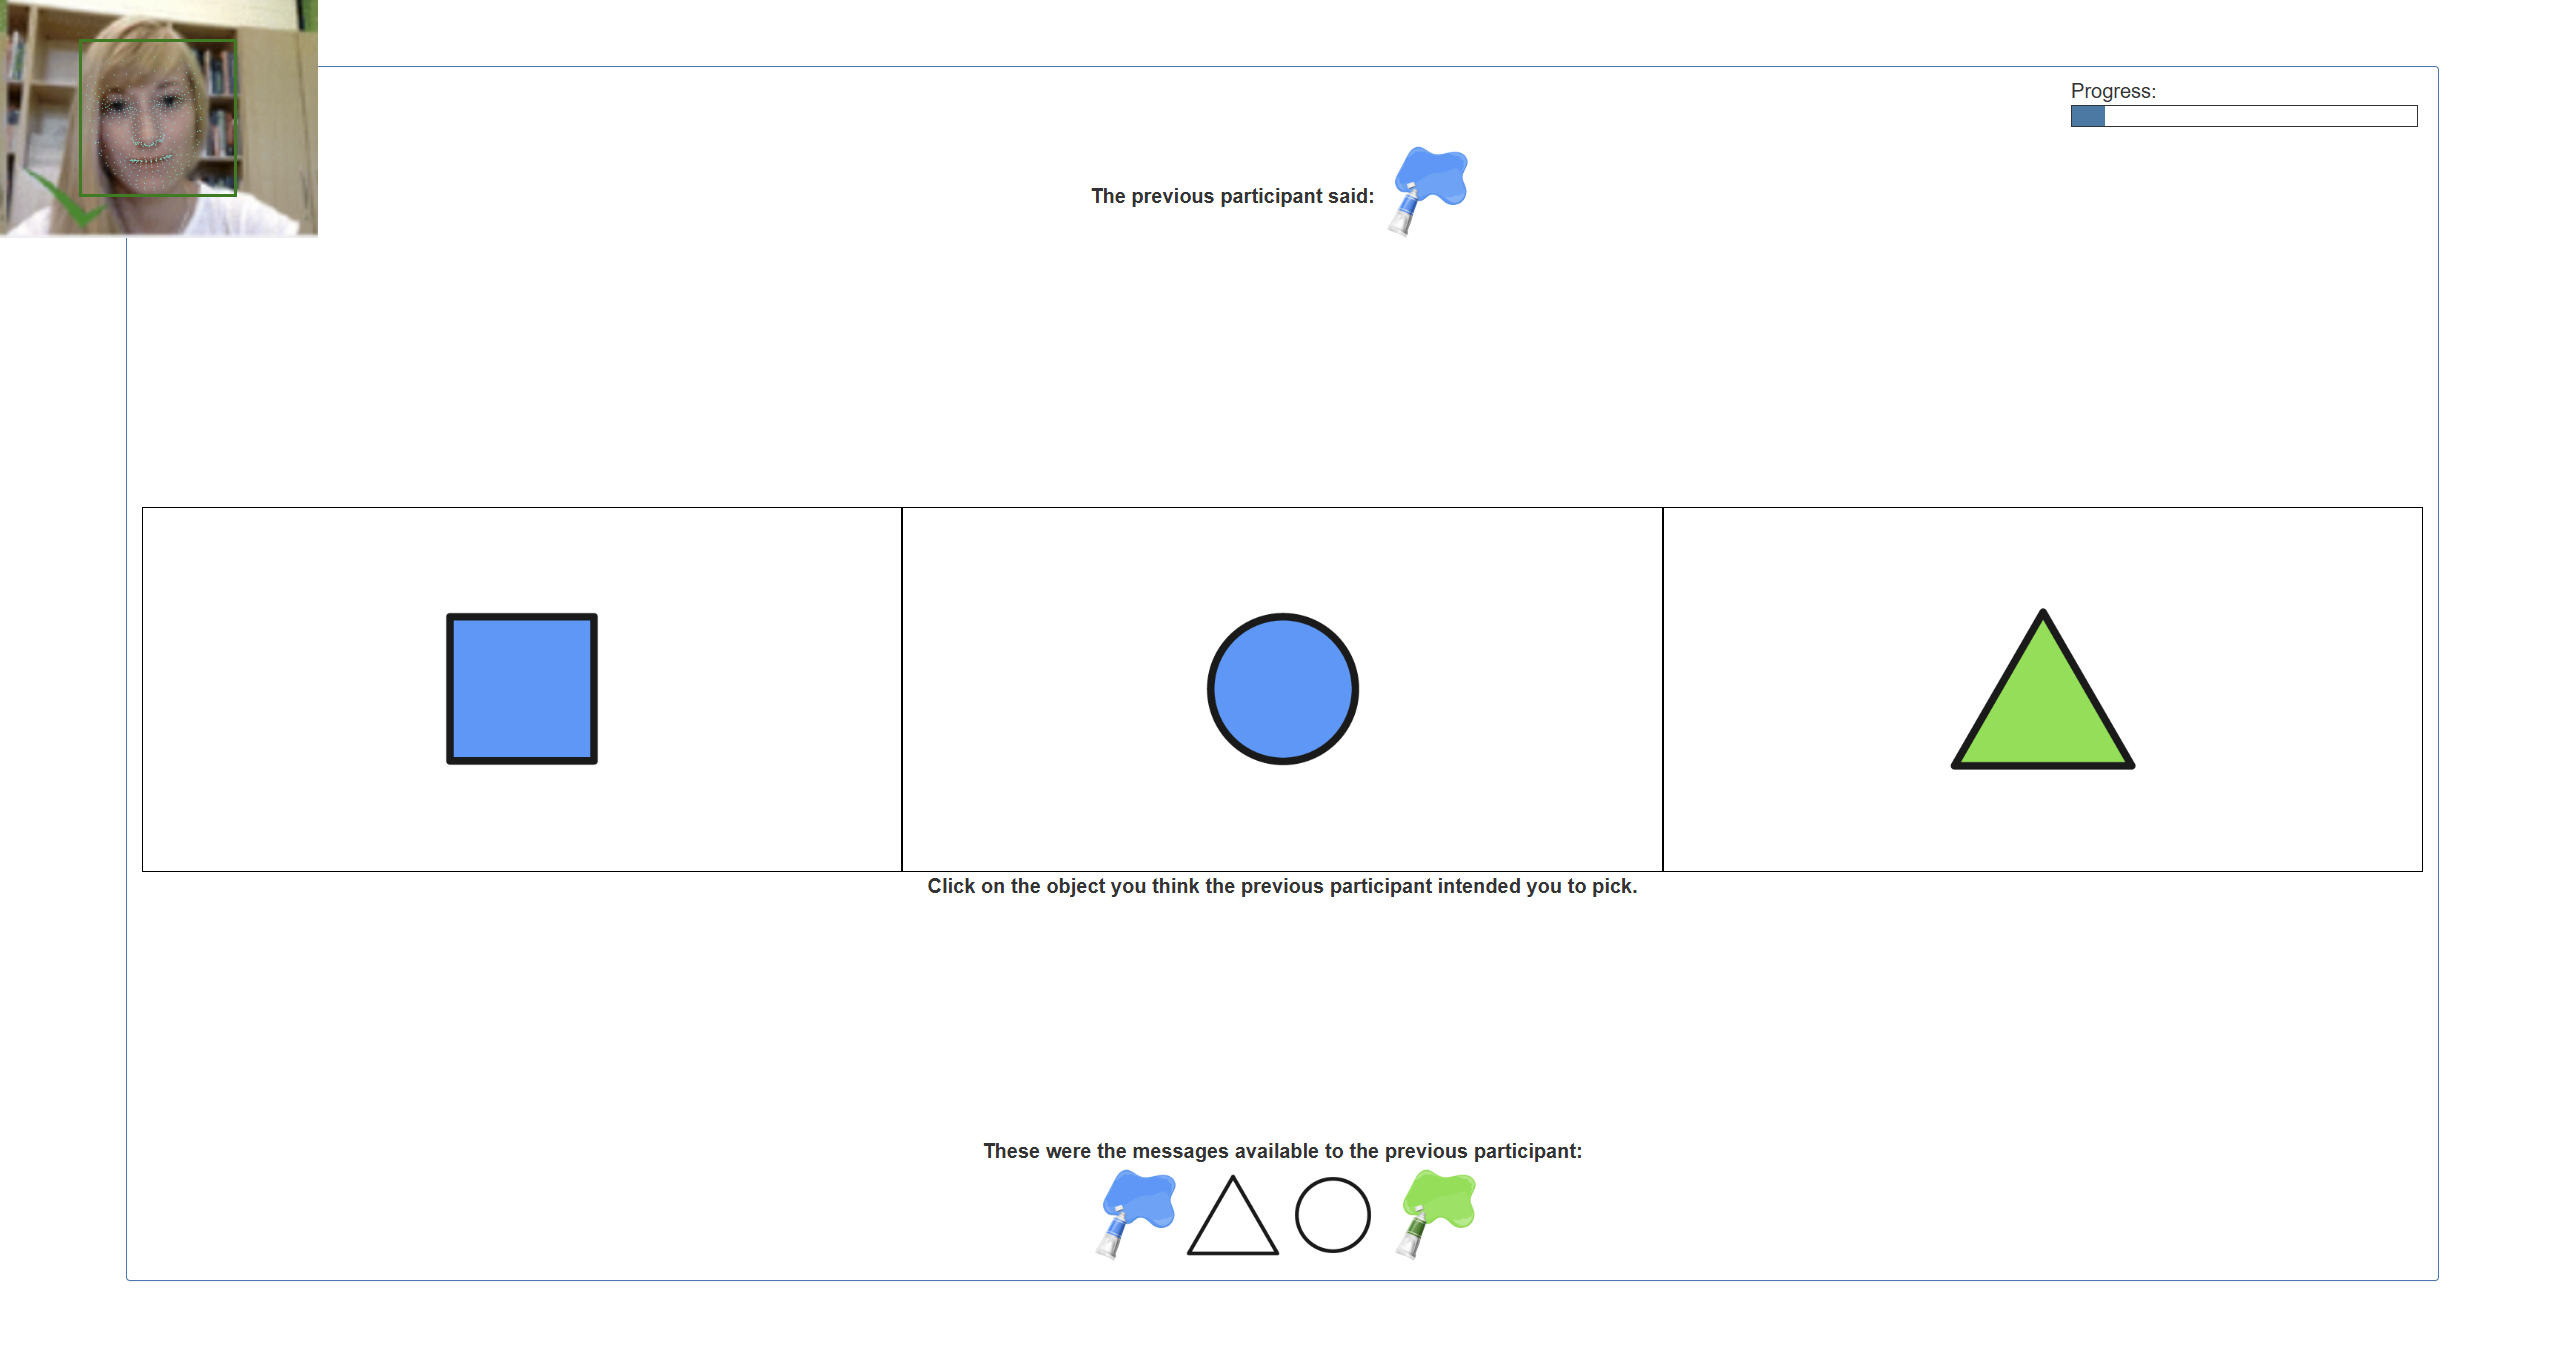
\includegraphics[width=0.8\textwidth]{images/example_trial_webcam.png}
    \caption{Example trial}
    \label{fig:example_trial_webcam}
\end{figure}

Before the main part of the experiment with 36 + 2 trials, the participants were asked to do a speaker's job in reference games with 3 Unambiguous trials and 1 completely ambiguous one. The participants were asked to describe the object in the ambiguous trial in a way that the listener would be able to pick the correct object. Later they were told that a previous participant had already done the speaker's job and they were to do the listener's job, which was the main part of the experiment with 36 + 2 trials. An example trial can be seen in \autoref{fig:example_trial_webcam}. Depending on the zoom and resolution on the page the sizes and absolute positions of the images would vary a lot. Hence, the absolute positions in pixels as well as sizes of the images were saved during the experiment. 

\subsection{Eye Tracking}
\label{sec:data:eyetr}
The eye tracking was done via library WebGazer \cite{wegbazer}. The library was used to track participants' gaze on the screen. There was a calibration in the beginning of the experiment after the practice trials where participants did the speaker's job, this allowed to put the calibration as close to the main experiment as possible. The calibration was adapted from the one used in the demo of WebGazer \cite{wegbazer}. Although, we included 11 points instead of 9, the additional points were put on the objects' places. Each point had to be clicked 5 times. The setup can be seen in \autoref{fig:calibration_webcam}.In addition, the calibration accuracy assessment in the end was done not with 1 point but 3: middle, left and right. Where left and right again correspond to the positions of the main objects on the screen. Furthermore, an in-between trial calibration was incorporated to ensure that the calibration was still accurate. The number of points were reduced to 5 each point corresponding to one of the areas of interest. No accuracy assessment was done during the in-between trial calibration. The setup can be seen in \autoref{fig:inbetween_calibration_webcam}.

\begin{figure}
    \centering
    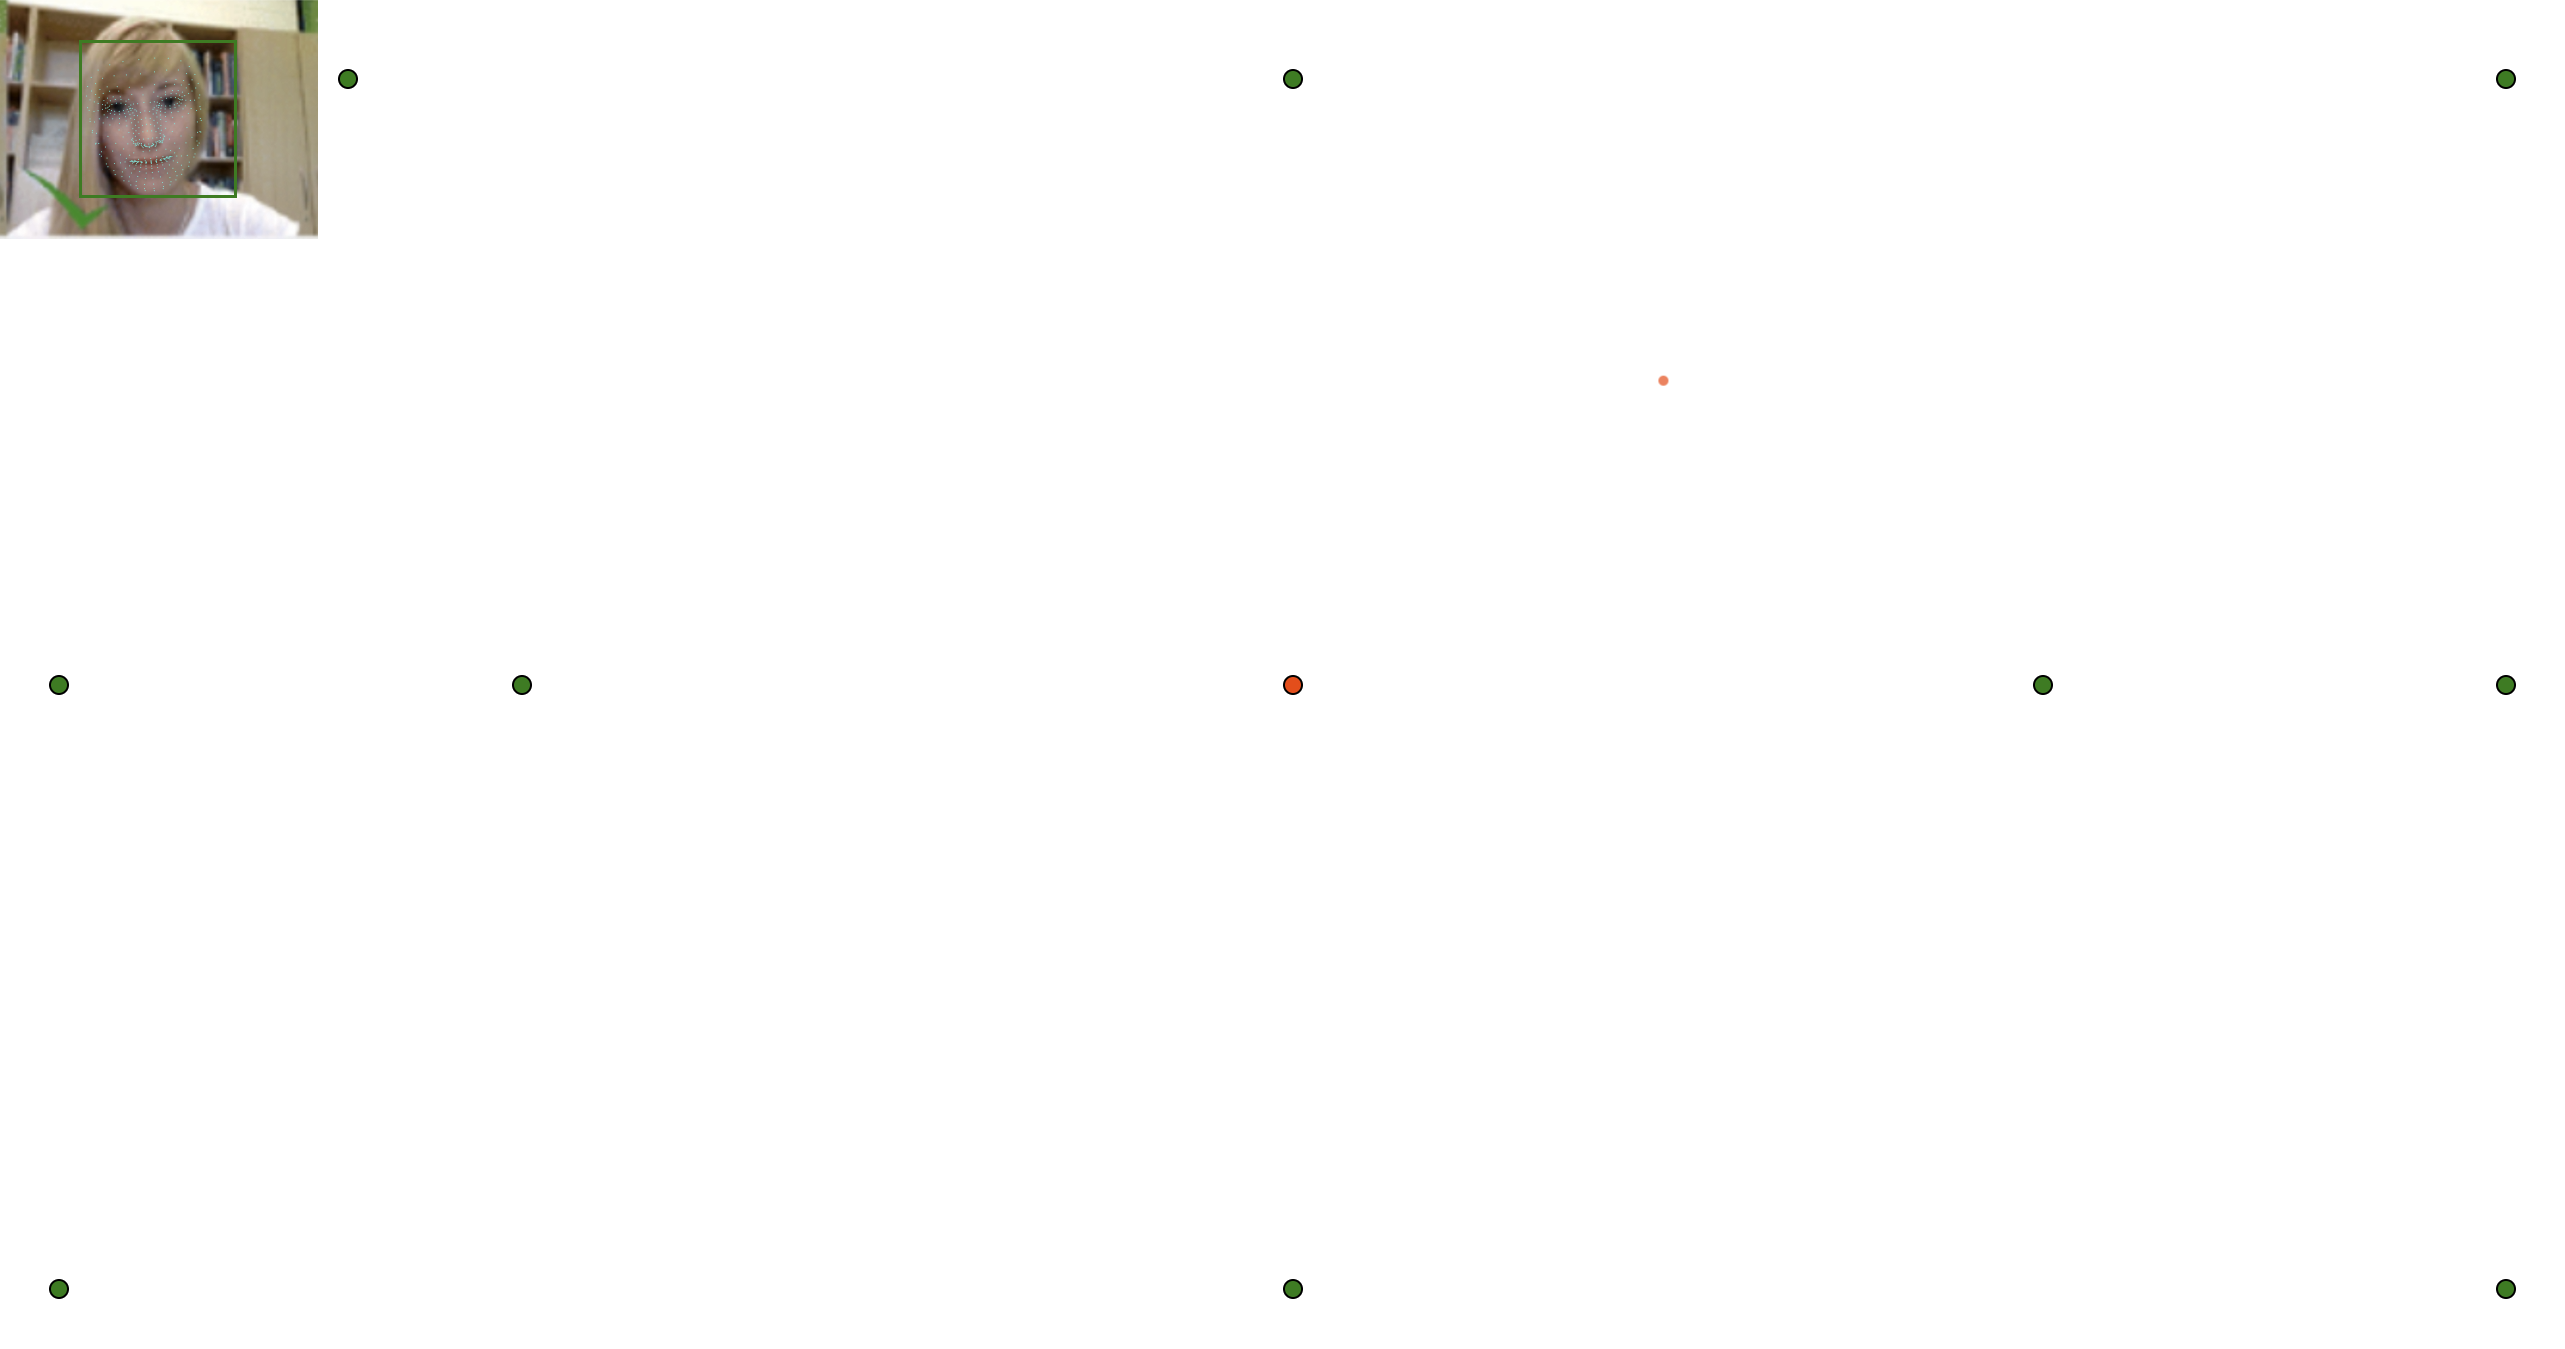
\includegraphics[width=0.8\textwidth]{images/calibration_webcam.png}
    \caption{Calibration setup}
    \label{fig:calibration_webcam}
\end{figure}

In order to successfully pass the calibration assessment, the participants must reach at least 65\% accuracy on each of the three calibration points. However, during the testing phase we noticed that the calibration assessment was too strict and difficult to pass. Therefore, it was decided to make the left and right points easier to calibrate via adjusting the calculation of the accuracy. A weighted accuracy calibration procedure was implemented. While the distance between for the accuracy of the middle point was calculated via euclidean distance, the left and right points were calculated via the following formula: $\sqrt{(w_x\cdot(calib\_point\_x - gaze\_x))^2 + (w_y\cdot(calib\_point\_y - gaze\_y))^2}$. Where $w_x$ and $w_y$ are the coefficients that were adjusted during the testing phase. The final values were $w_x = 1$ and $w_y = 0.5$. The values were chosen based on the fact that left and right objects do not have any other objects on the vertical axes this can be seen in \autoref{fig:example_trial_webcam}. Therefore a slightly inaccurate result on the vertical axes would be relatively easy to correct during the analysis.

The images were located on the screen as far as possible to reduce the errors as much as possible. For the same reason, the sent message were kept as a single block instead of being spread further apart. 

Furthermore, a performance issue arised during the pilot phase. The issues was that the eye tracking became very slow and laggy towards the the second half of the experiment. The more clicks were made, the worse the performance became. Due to a drastic drop in sampling rate and increase in response time, the pilot data was clearly unacceptable. The issue was resolved by reducing the \text{DataWindow} size from 700 to 50 in source code and recreating the WebGazer source file afterwards. The issue was resolved and the performance was stable throughout the experiment. 

\begin{figure}
    \centering
    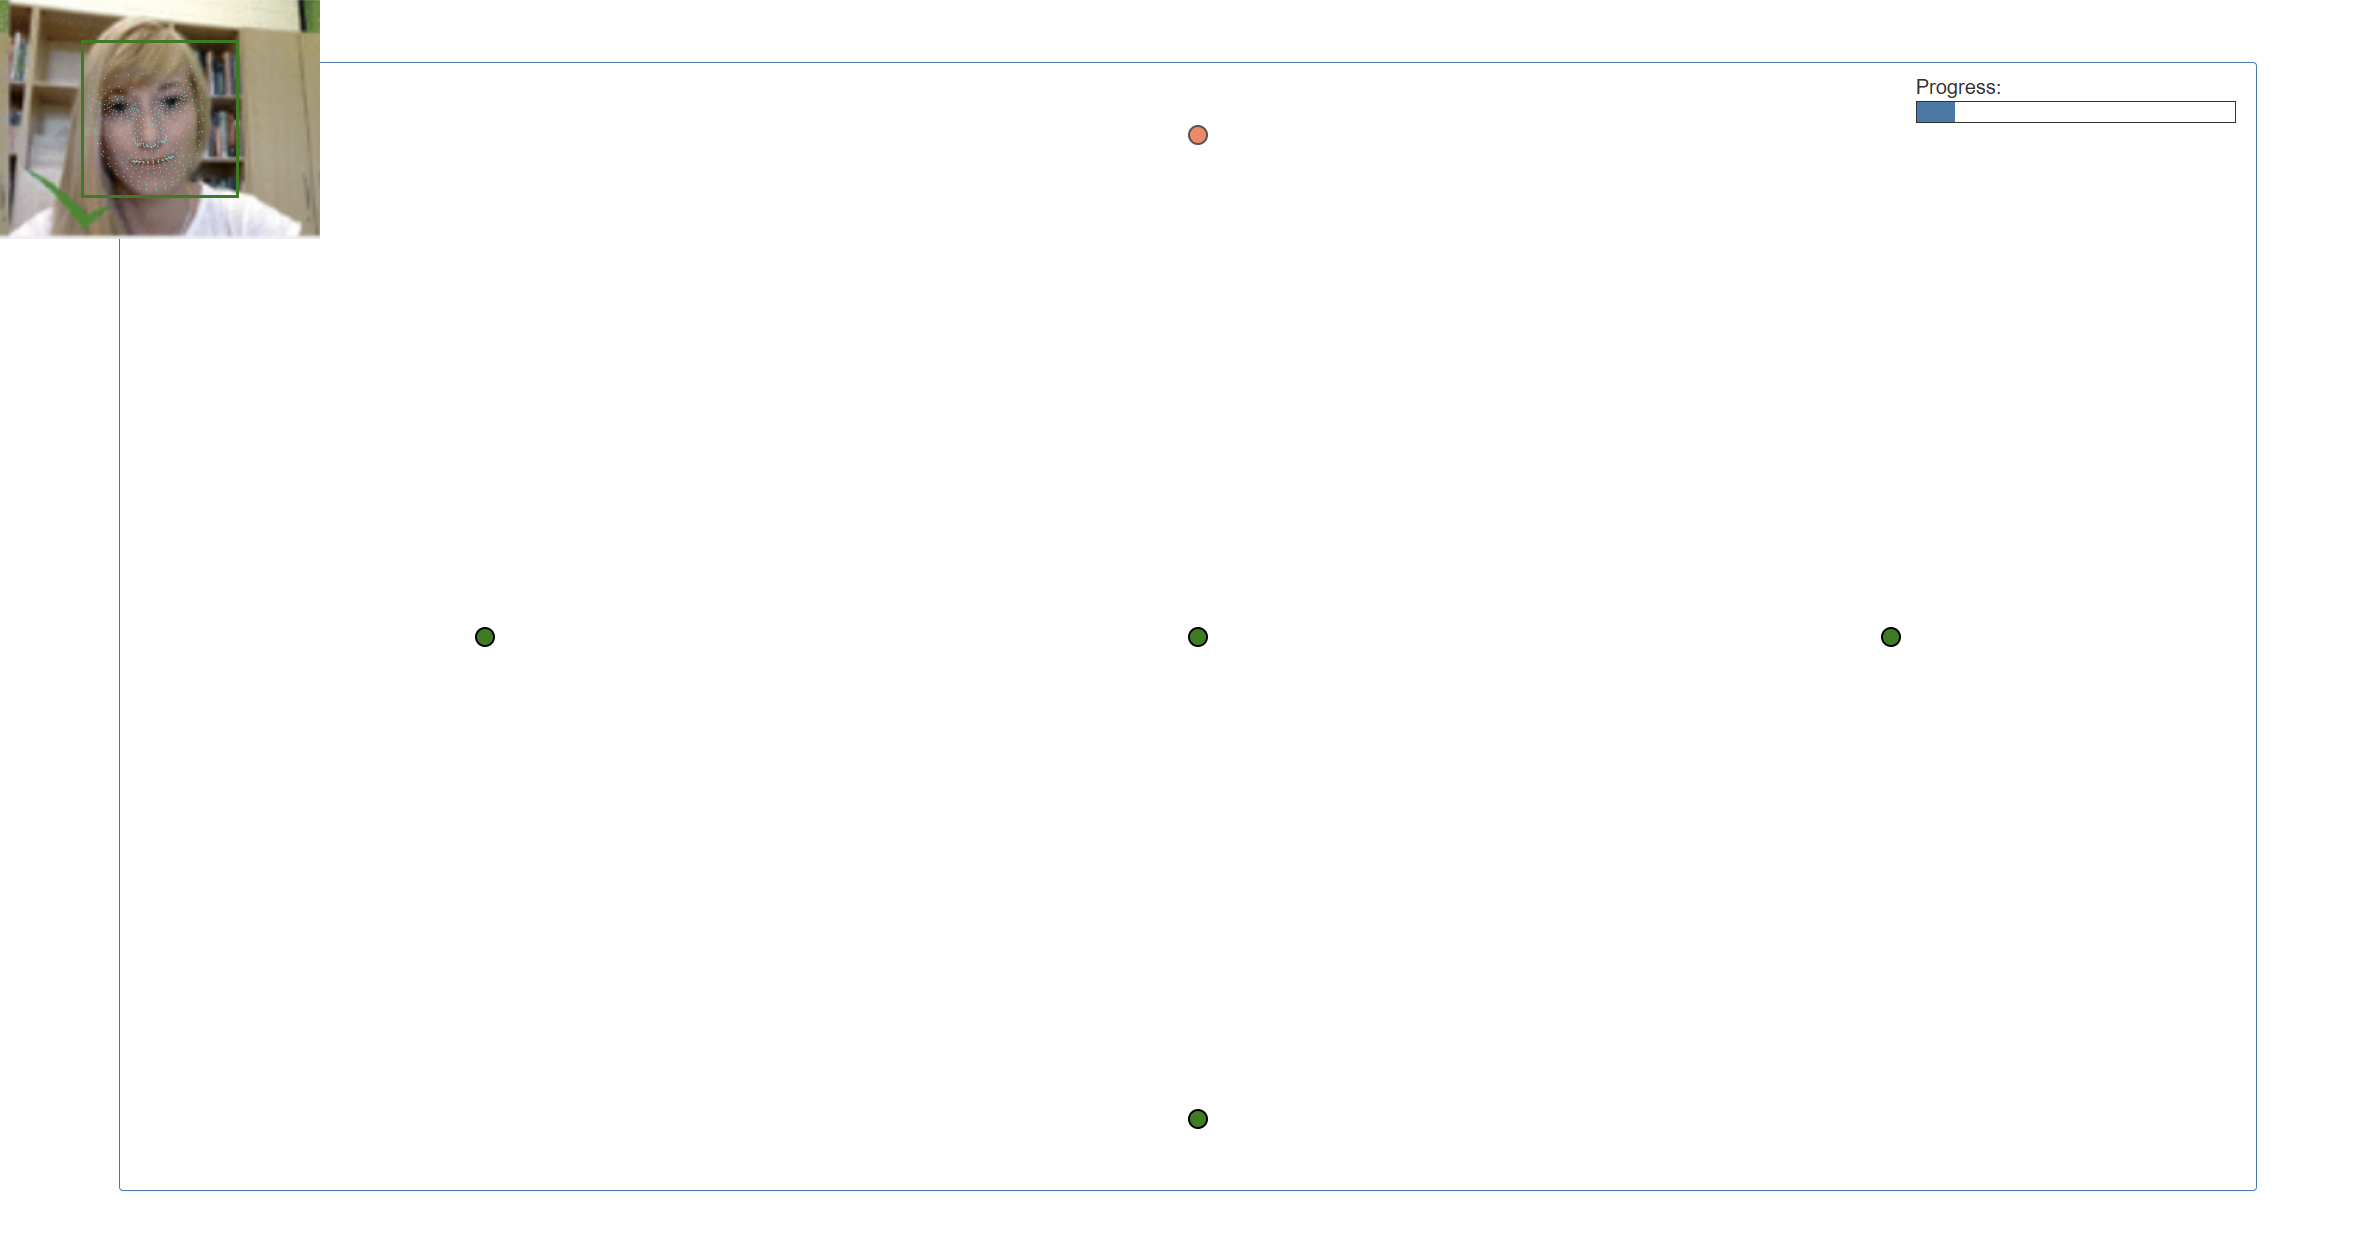
\includegraphics[width=0.8\textwidth]{images/inbetween_calibration_webcam.png}
    \caption{In-between trial calibration}
    \label{fig:inbetween_calibration_webcam}
\end{figure}

\begin{figure}
    \centering
    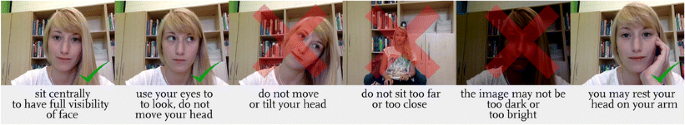
\includegraphics[width=0.8\textwidth]{images/calibration_instr.png}
    \caption{Calibration instructions taken from \cite{Semmelmann_2018}}
    \label{fig:calibration_instr}
\end{figure}

The calibration is highly dependent on the setup. Hence, the following pieces of advice were given to the participants to increase chances of successful calibration: keep the laptop on charging during the whole experiment (to make sure the eye tracking does not suffer from battery saving features); choose a quiet, well-lit room with minimal distractions and use a stable chair; place your laptop on a stable surface, screen directly in front of you. Later during the calibration, ensure the webcam is centered with your face; keep your head sas still as possible during the experiment; make this window full screen size if not already. In addition, right before the calibration the participants were shown their webcam feed to make sure they are centered and the lighting is good as well as some visual advice on how to improve the calibration. The visuals can be seen in \autoref{fig:calibration_instr}. They were taken from a different experiment \cite{Semmelmann_2018} that was conducted with use of WebGazer \cite{wegbazer}.

Even with all the optimizations in place, the calibration procedure was still relatively difficult to pass. The participants were not restricted in number of attempts to calibrate. However, the participants were informed that the approval is only possible after successfully completing the calibration and the rest of the experiment. The resulting rate of successful completions was only around 30\%. However, that resulted in a good quality of data.

\subsection{Consent}
The participants were told about the eye tracking right in the beginning of the experiment. They were informed that no video of them will be stored at any point of time. The participants were informed that they can stop the experiment at any point by exiting the website and none of their data will be saved. The exact formulation was: 

\begin{quote}
    This experiment is being conducted as part of ongoing research at Saarland University. If you have any questions or comments about the study, please contact us. You must be at least 18 years old to participate. Your participation in this research is voluntary. There are no risks or benefits to participating in this study. You may decline to answer any or all of the following questions. You may decline further participation, at any time, without adverse consequences. Part of the data collections involves using your webcam to estimate your eye gaze. No video or audio is stored at any point during the experiment. We only use the video to store the estimated position of your eye gaze, as well as estimated size of your pupil. All data will be anonymized prior to analysis. 

    If you agree to participate, please read the below instructions before proceeding.
\end{quote}


\section{Analysis}
\label{sec:analysis}

\subsection{Features}
\label{sec:analysis:features}
Considering the related eye tracking study \cite{Vigneau_2006}, the analysis will be around the defined eye tracking features. \cite{Vigneau_2006} defined mainly 5 types of features: absolute time on an area of interest, proportional time on an area of interest, toggling (between the Raven's matrix and the available messages), item latency (time to complete the trial) and latency to first toggle and matrix distribution index (how equally the attention was spread across the matrix items). In this study on the other hand, we are mainly focused on the proportional time on the areas of interest. The decision was made for multiple reasons. First of all the sampling rate of WebGazer is highly dependent on the participants' computer, making the absolute time on the areas of interest and latency to first fixation not comparable between participants. Second of all, we do not have such a strong hypothesis about what exactly people do during the task solving process as \cite{Vigneau_2006} had. We are rather interested in the general profile of attention, hence, no toggling features were included in the analysis. 

In addition to the eye tracking features, we included some general features about the trial. The features are: trial number, condition (Simple, Complex, Unambiguous), type of sent message feature (shape or color), correct (whether the trial was solved correctly or not) and target position (left, center or right). The condition and correct features play crucial role in the analysis. While the other features such as trial number, type of sent message and target position were included due to the fact that they were shown to have a significant effect on the participants' performance in the previous studies \cite{Mayn_2023, Mayn_2025}.

\subsection{Data Preprocessing}
\label{sec:analysis:preprocessing}


\subsection{Pairwise Correlations}
\label{sec:analysis:corr}

\subsection{Mixed Effects Logistic Regressions}
\label{sec:analysis:mixed_effects}

\subsection{Exploratory Analysis}
\label{sec:analysis:exploratory}

\subsubsection{Clustering}
\label{sec:analysis:exploratory:clustering}

\subsubsection{CNNs}
\label{sec:analysis:exploratory:cnn}
